\section{Introduction}
\section{Background and Motivation}
\improvement{Compartiment in subsections to improve narrative flow}
\subsubsection*{Origins, promise and challenges of blockchain technology}
The advent of blockchain technology since the launch of Bitcoin in 2009 has sparked a revolution in systems of value transfer, transparency, and decentralization \cite{nakamotoBitcoinPeertopeerElectronic2008}. However, the early meteoric rise of cryptocurrencies and underlying blockchain networks has raised critical concerns regarding their environmental sustainability. With the benefit of hindsight, we can view this period as Gartner's Peak of Inflated Expectations. Now, with notorious founders imprisoned, increasing regulatory scrutiny, and the total cryptocurrency market capitalization down
XX\% from its peak \change{cite}, the blockchain ecosystem stands at a crossroads. This is an opportunity to refocus on the core propositions of blockchain technology and ensure its long-term viability.


The dominant network, Bitcoin, which utilizes a computationally-intensive proof-of-work consensus mechanism, has attracted particular scrutiny for its high energy consumption. Recent estimates indicate the Bitcoin network alone may consume between 115 and 150 TWh annually, comparable to entire countries like the Netherlands \cite{devriesRevisitingBitcoinCarbon2022,neumuellerCambridgeBitcoinElectricity2021}. This growing apetite for energy competes with the just starting energy transition, putting electrical production and distribution networks under stress. Finally it also results in significant CO2 emissions, hardly compatible with global climate goals like the Paris Climate Accords.

\subsubsection*{Limitations of current approaches}
However, we must recognize the complexity and nuance when evaluating blockchain sustainability. Consensus protocols, design choices, and use cases vary greatly across different networks, leading to wide variability in energy needs and emissions. For instance, proof-of-stake networks like Cardano and Solana promise energy savings by factors of 1000x or more compared to proof-of-work \cite{kohliAnalysisEnergyConsumption2023}. Moreover, Ethereum recently completed its highly anticipated, technically and politically complex transition from proof-of-work to proof-of-stake, demonstrating that such migrations are viable for major networks. \cite{EthereumMergeYour2022} The nascent field of blockchain sustainability analysis must evolve more granular, differentiated perspectives.

Initial responses from the blockchain industry have focused on high-level aggregate comparisons and rankings between networks. For example, recent benchmarks like the Crypto Carbon Ratings Institute methodology provide standardized comparisons of the total lifecycle emissions across chains [5]. However, these overlook the diversity of users and fail to provide accountability at an individual level.

This poses a critical gap, especially as blockchain technology expands into mainstream adoption. We lack a methodology to attribute network-wide emissions to specific users based on their unique activity patterns and values. Such granular carbon accounting can raise awareness of individual impact and empower ethical participation.

\subsubsection*{Opportunities for user-level footprinting}

To address this, the novel approach in this thesis involves an attribution model that weighs factors like asset holdings, transactions, and computations based on their estimated importance to users on each chain. By considering relative user perspectives, we can map emissions more accurately to individual entities like protocols, DAOs, or end-users. This unconventional yet powerful approach unlocks new potentials for transparency, responsibility, and sustainability.

\begin{figure}[hbt!]
    \centering
    \centerline{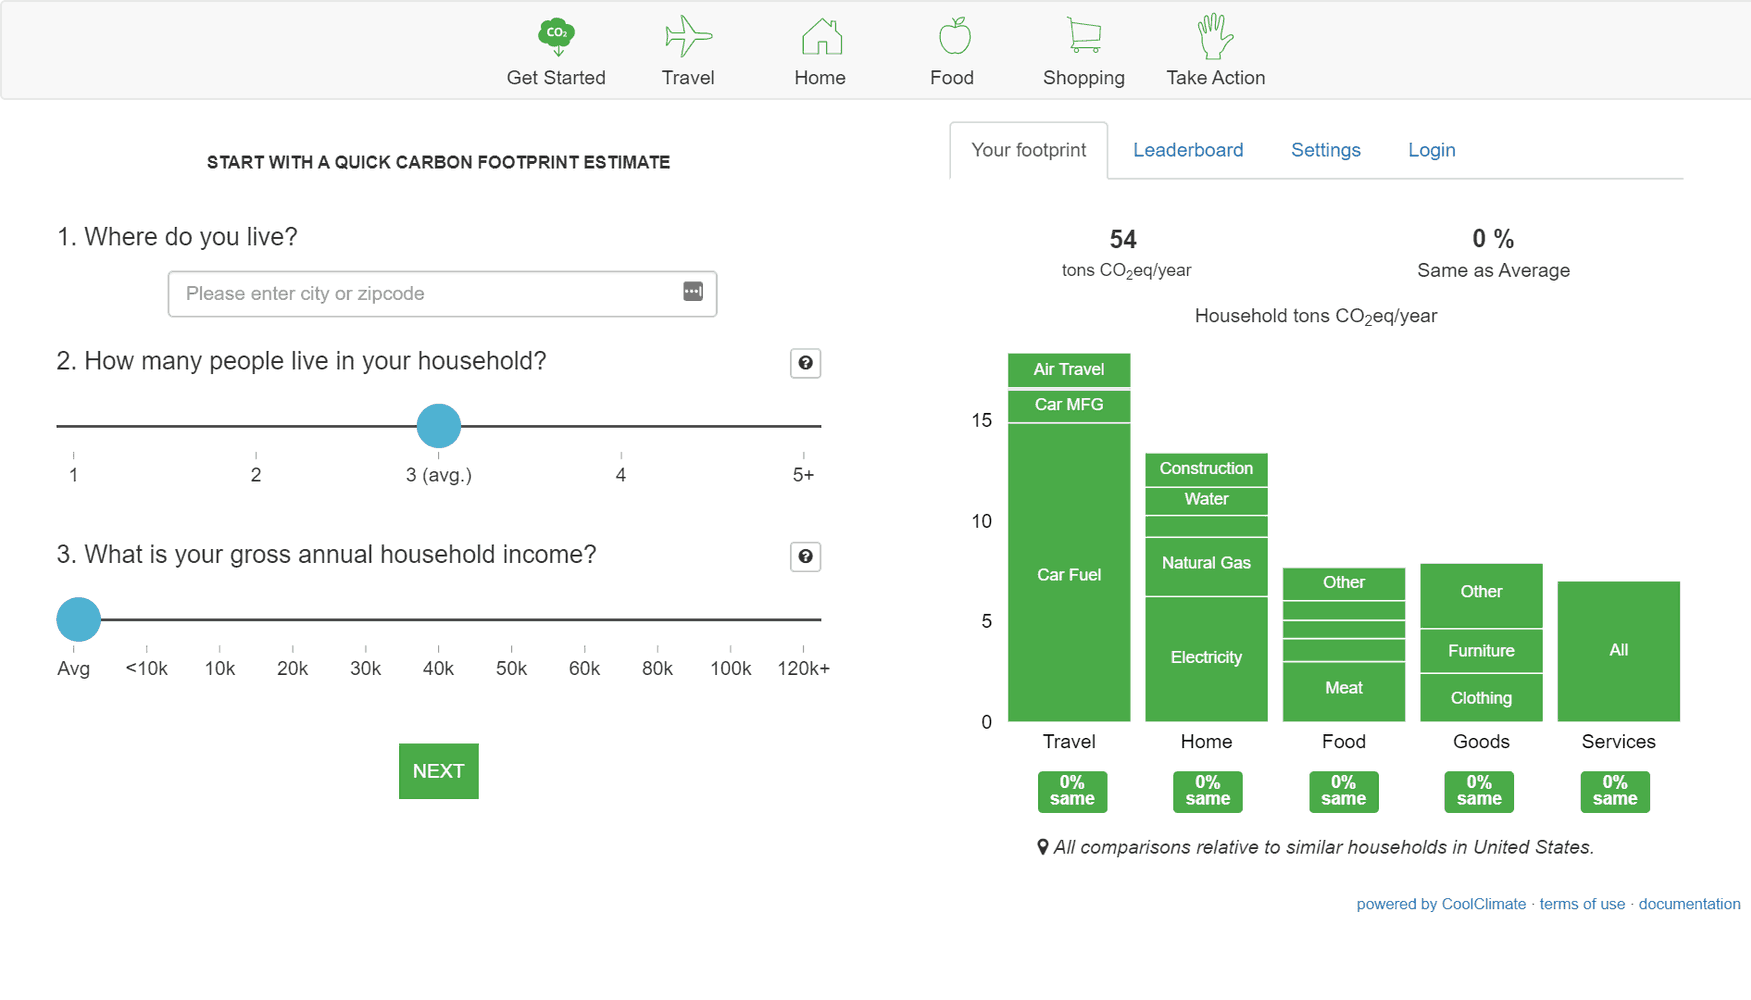
\includegraphics[scale=0.25]{figures/carbon_footprint_calculator.png}}
    \caption[YO]{Tradionnal carbon footprint calculator form - CoolClimate\footnotemark}
    \label{fig:carbon_footprint_calculator}
\end{figure}

\footnotetext{https://coolclimate.org/calculator}

Limited User engagement towards footprint calculators, tedious process and error prone \cite{saloOpportunitiesLimitationsCarbon2019,mulrowStateCarbonFootprint2019}.

\todo{This is the user experience that will be improved with blockchain data transparency and attribution. Link wiht further use sustainability use cases. Blockchain based footprints makes possible automating the process and vastly increases accuracy as it is no more a self assesment. Cite issues of carbon footprint calculator accuracy because of self assesment.}
\section{Problem Statement}

As blockchain technology progresses into mainstream integration, the lack of transparency and accountability for emissions at an individual user level poses a critical gap. For example, retail investors drawn to crypto assets may be unaware of the passive environmental impacts associated with their portfolios over time. There is also increasing offering of decentralized applications (web3) with usage beyond those of investing. Granular carbon accounting and attribution to individual wallets can raise awareness and enable offsetting as a means for users to take responsibility of their actions.

Moreover, this gap becomes even more complex for providers of decentralized apps or decentralized autonomous organizations (DAOs) comprising multiple smart contracts and user addresses. Without a methodology for attributing network-wide emissions based on collective usage patterns, a DAO cannot fully assess and mitigate its overall carbon footprint.

Therefore, the overarching problem this thesis addresses is:

"How can we design an attribution model that allocates the carbon emissions of any blockchain network to specific user entities or addresses in a transparent, accurate, and relevant manner based on their unique activity patterns?"


\section{Research Questions and Ojbectives}

To systematically address the problem of transparent and accurate carbon attribution for blockchain users and entities, this thesis pursues four key research questions:

\begin{enumerate}
    \item How can blockchain emission factors be quantified at a granular, user-centric level, beyond aggregate network-wide estimates?
    \item What are appropriate metrics and weighting systems to reflect the responsibilities of diverse blockchain users based on their activities?
    \item How can we validate and demonstrate such an attribution model through a practical implementation?
    \item What are the broader implications of user-centric emissions accounting for accelerating sustainability as blockchain technology matures?
\end{enumerate}

The main objectives of this work are:

\begin{description}

    \item [Develop a User-Level Attribution Model] \hfill \\
          Develop a robust emissions attribution methodology based on usage and responsibility.
    \item [Greenblock: Pratical Application] \hfill \\
          Implement and validate the model through a functional proof-of-concept application.
    \item [Promote awareness and Responsibility] \hfill \\
          of environmental impact among blockchain users.
    \item [The Future of Sustainability and Blockchain] \change{to complete}
\end{description}
